\section{Vorbereitungsaufgabe}

\subsection{Auflösungsvermögen und Dispersionsgebiet der Lummer-Gehrcke-Platte}
Nach den Gleichungen \ref{eq:dispersionsgebiet} und \ref{eq:auflösungsvermögen} lassen sich nun das Dispersionsgebiet und das Auflösungsvermögen der Lummer-Gehrcke-Platte für die rote ($\lambda=\SI{643,8}{\nano\meter}$) und die blaue ($\lambda=\SI{480}{\nano\meter}$) Linie berechnen (siehe Tabelle \ref{tab:auflösungsunddispersion}). Die Berechnung erfolgt dabei mit $d=\SI{4}{\milli\meter}$, $L=\SI{120}{\milli\meter}$, $n($rot$)=1,4567$, $n($blau$)=1,4635$.
	
\begin{table}[htpb]
	\centering
	\caption{Bestimmung des Auflösungsvermögens $A$ und des Dispersionsgebiets $\Delta\lambda_\text{D}$.}
	\label{tab:auflösungsunddispersion}
	\begin{tabular}{c c c}
		\toprule
		& $\lambda_\text{D} / \si{\pico\meter}$ & $A$ \\
		\midrule
		rot & 48,91 & 209129 \\
		blau & 27,0 & 285458 \\ 
		\bottomrule
	\end{tabular}
\end{table}

\subsection{Termschemata der Spektrallinien}

Die rote Linie entspricht einem Übergang $^1P_1\longleftrightarrow\,^1D_2$, die blaue $^3S_1\longleftrightarrow\,^3P_1$. Die Quantenzahlen und die nach Gleichung \eqref{eqn:lande} berechneten Landé-Faktoren der einzelnen Zustände sind aus der Tabelle \ref{tab:lande} zu entnehmen.
Die Termschemata befindet sich in der Abbildung \ref{fig:termschemata}. 
\begin{table}[h!]
	\centering
	\begin{tabular}{r|rrr|r}
		\hline\hline
		Zustand & $L$	&	$S$	&	$J$	&	$g_J$\\
		\hline\hline
		$^1P_1$ &	1	&	0	&	1	&	1\\
		$^1D_2$ &	2	&	0	&	2	&	1\\
		$^3S_1$ &	0	&	1	&	1	&	2\\
		$^3P_1$ &	1	&	1	&	1	&	$\frac{3}{2}$\\
		\hline
	\end{tabular}
	\caption{Die ausgerechneten Landé-Faktoren.}
	\label{tab:lande}
\end{table}

Für die Aufspaltung der Zeeman-Linien ergeben sich damit unter Beachtung von Gleichung \ref{eqn:Eanomal} die Energieunterschiede in Tabelle \ref{tabenergy}. Die Energiedifferenz ergibt sich dann zu:
\begin{equation}
\Delta E = g_{ij} \mu_\text{B} B
\end{equation}
wobei $g_{ij} = m_ig_i-m_jg_j$.
\begin{table}[h]
	\begin{center}
		\begin{tabular}{c|ccc}
			&$\Delta m = -1$&$\Delta m = 0$&$\Delta m = +1$ \\ \hline
			rot & $\mu_{\text{B}} B$ & $0$ & $- \mu_{\text{B}} B$ \\
			blau ($m_1=+1$) & $\frac{3}{2} \mu_{\text{B}} B$ & $-\frac{1}{2} \mu_{\text{B}} B$ & - \\
			blau ($m_1=0$) & $2 \mu_{\text{B}} B$ & 0 & $-2 \mu_{\text{B}} B$ \\
			blau ($m_1=-1$) & - & $\frac{1}{2} \mu_{\text{B}} B$ & $-\frac{3}{2} \mu_{\text{B}} B$
		\end{tabular}
		\caption{Energieniveauunterschiede $\Delta E$ für ausgewählte Niveaus für $643{,}8\text{ nm}$ (rot) und $480 \text{ nm}$ (blau).}
		\label{tabenergy}
	\end{center}
\end{table}

\begin{figure}[h!]
	\centering
	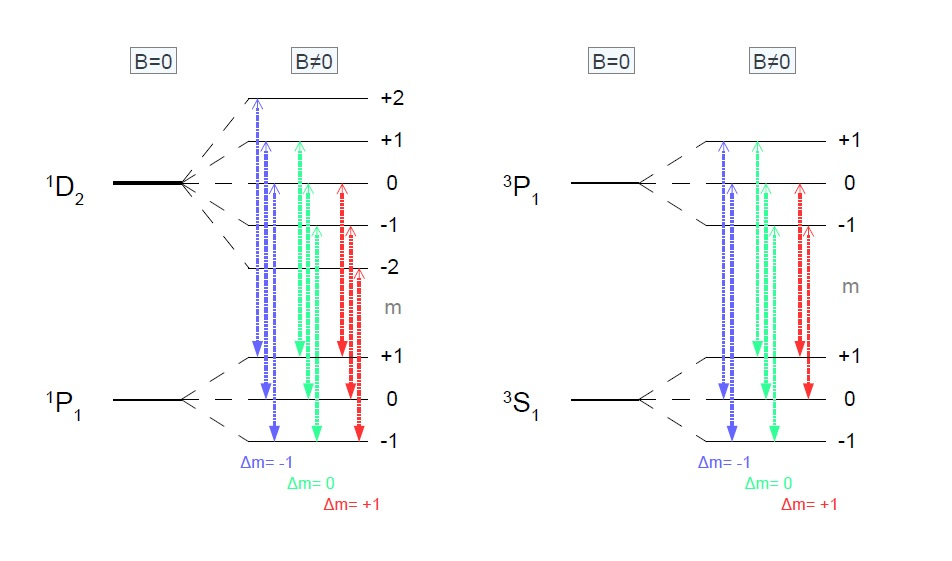
\includegraphics[width=0.9\linewidth]{content/Termschemata}
	\caption{Die Termschemata und die möglichen Übergänge, \cite[5]{termschemata}.}
	\label{fig:termschemata}
\end{figure}

\section{Auswertung}
\label{sec:Auswertung}


